% Section content template for individual Educative lessons
% This file contains the actual content for a specific section
% Generated from Educative API section content

% Section: Sequence Diagram for  Facebook
% Section ID: 5720196763615232
% Section Slug: sequence-diagram-for-facebook
% Generated: 2025-12-14T12:40:09.106774

Sequence diagrams are a great way to understand the interactions between different entities and objects in the system. There can be different sequence diagrams that we can create for Facebook. In this lesson, we will create sequence diagrams for the following interaction:

\begin{itemize}
\item
\protect\phantomsection\label{jKkzImlT3YpPqKRKuqLR2}
\textbf{Send a friend request:} A user sends a friend request to another user.
\end{itemize}

\subsection{Send a friend request}\label{3FS_rdA0ggKzHzgmO6D-T}
\\
The sequence diagram for sending a friend request should have the following actors and objects that will interact with each other:

\begin{itemize}
\item
\protect\phantomsection\label{JwdMtPRxzhyvMYQlz5L6S}
\textbf{Actors:} User\ A and User\ B
\item
\protect\phantomsection\label{X0q9EZJUomfO9B2pr7Zmx}
\textbf{Objects:} \texttt{Catalog} and \texttt{FriendRequest}
\end{itemize}
\\
Here are the steps for the ``send a friend request'' interaction:

\begin{enumerate}
\item
\protect\phantomsection\label{Wvi9yr2Ttm1q8HHPWivKP}
User A searches for user B in the catalog.
\item
\protect\phantomsection\label{cR6MjmbW7DkcZnKreQQf7}
If User B exists:

\begin{enumerate}
\item
The catalog returns user B
\item
User A adds user B as a friend.
\item
The friend request is sent to user B.
\item
If the request is accepted:

\begin{enumerate}
\item
User B is added to user A's friend list.
\item
User A is notified that the friend request has been accepted.
\end{enumerate}
\item
Otherwise, the request is rejected.
\end{enumerate}
\item
\protect\phantomsection\label{xSAN6UAS7X0ANPjOCxf58}
Else, if user B does not exist:

\begin{enumerate}
\item
User A receives a ``user not found'' error.
\end{enumerate}
\end{enumerate}
\\
Based on the order above, the sequence diagram for sending a friend request on Facebook is given below:

\begin{figure}[htbp]
 \centering
 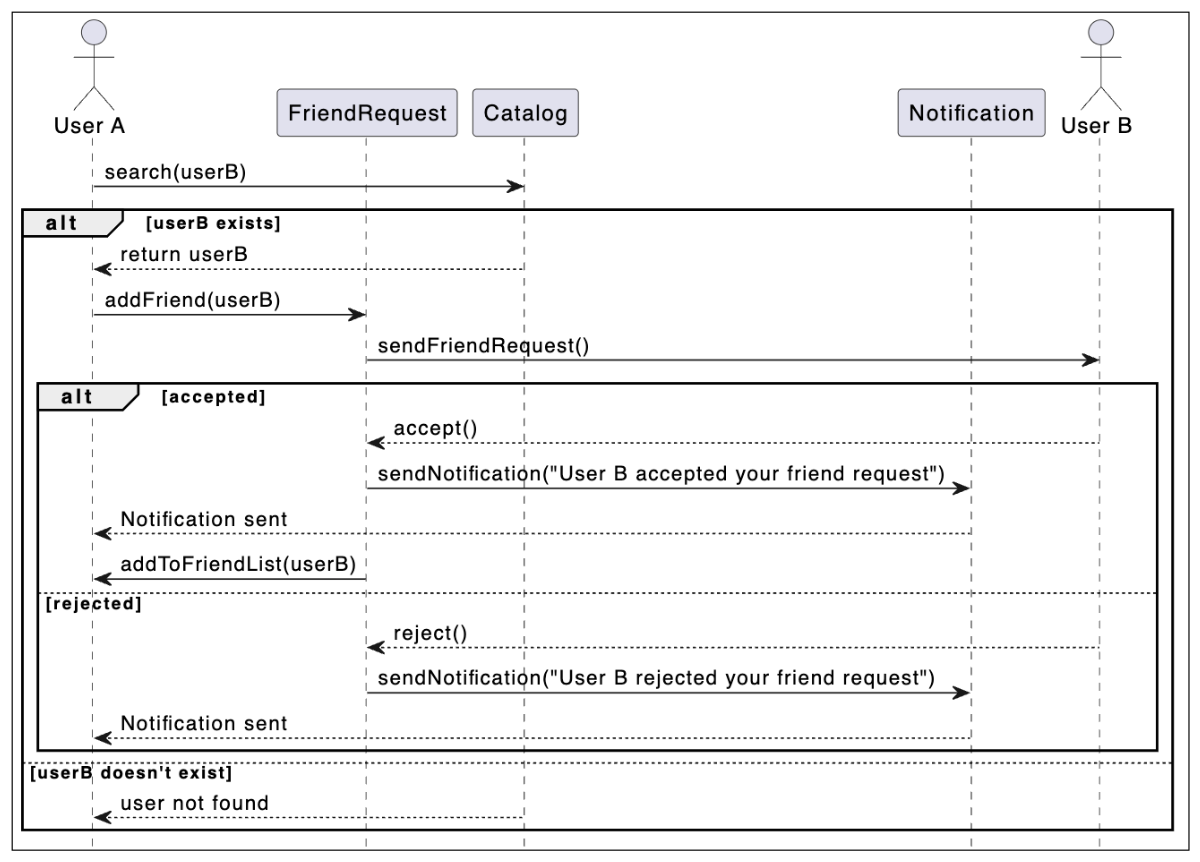
\includegraphics[width=0.5\textwidth]{Images/chapter_22/section_5720196763615232/4738782250008576.png}
 \caption{The sequence diagram for sending a friend request}
\end{figure}

Next, let's look at the activity diagrams for Facebook to understand the control flow of the system.

% End of section content